\section{The PDF Trust Chain \note{1.5pp}}
\label{sec:trust-chain}

\subsection{Trust Chains, Abstractly}

The term \emph{Trust Chain} (or ``Chain of Trust'') is used in multiple contexts, e.g.,
\emph{digital certificates}: a sequence of certificates signing certificates,
starting with a root certificate;
\emph{supply chain}: a product is no more reliable or secure as its
outsourced components;
\emph{trusted boot}: unless the bootloader is correct and non-malicious,
there can be no possibility of the operating system being the same;
\emph{software stacks}: upper layers are dependent upon lower layers (such as
system libraries) and vulnerabilities at the bottom affect all layers above.

The common idea is having layers
that rely on lower layers for their validity
(or components that rely on sub-components, etc.)
And the key lesson being,
{\bf{if a single layer of the trust chain 
  is flawed or suborned, then every layer relying on it
  is no longer capable of being trusted.}}

\subsection{The Trust Chain of a PDF Parser}

\todo{terminology: use layer}

% In \cref{sec:pdf-challenges}, we elaborated on the challenges of PDF.
% Parsing data-formats has a long history and many solutions ...
% Parsing formal languages also has a long history and many solutions ...
% PDF has aspects of both: this makes PDF challenging.
% But PDF ``parsing'' is not merely a matter of harder [difference of degree]
% but intrinsically more complex [a difference of kind!]:

\begin{figure}[t]
    \centering
    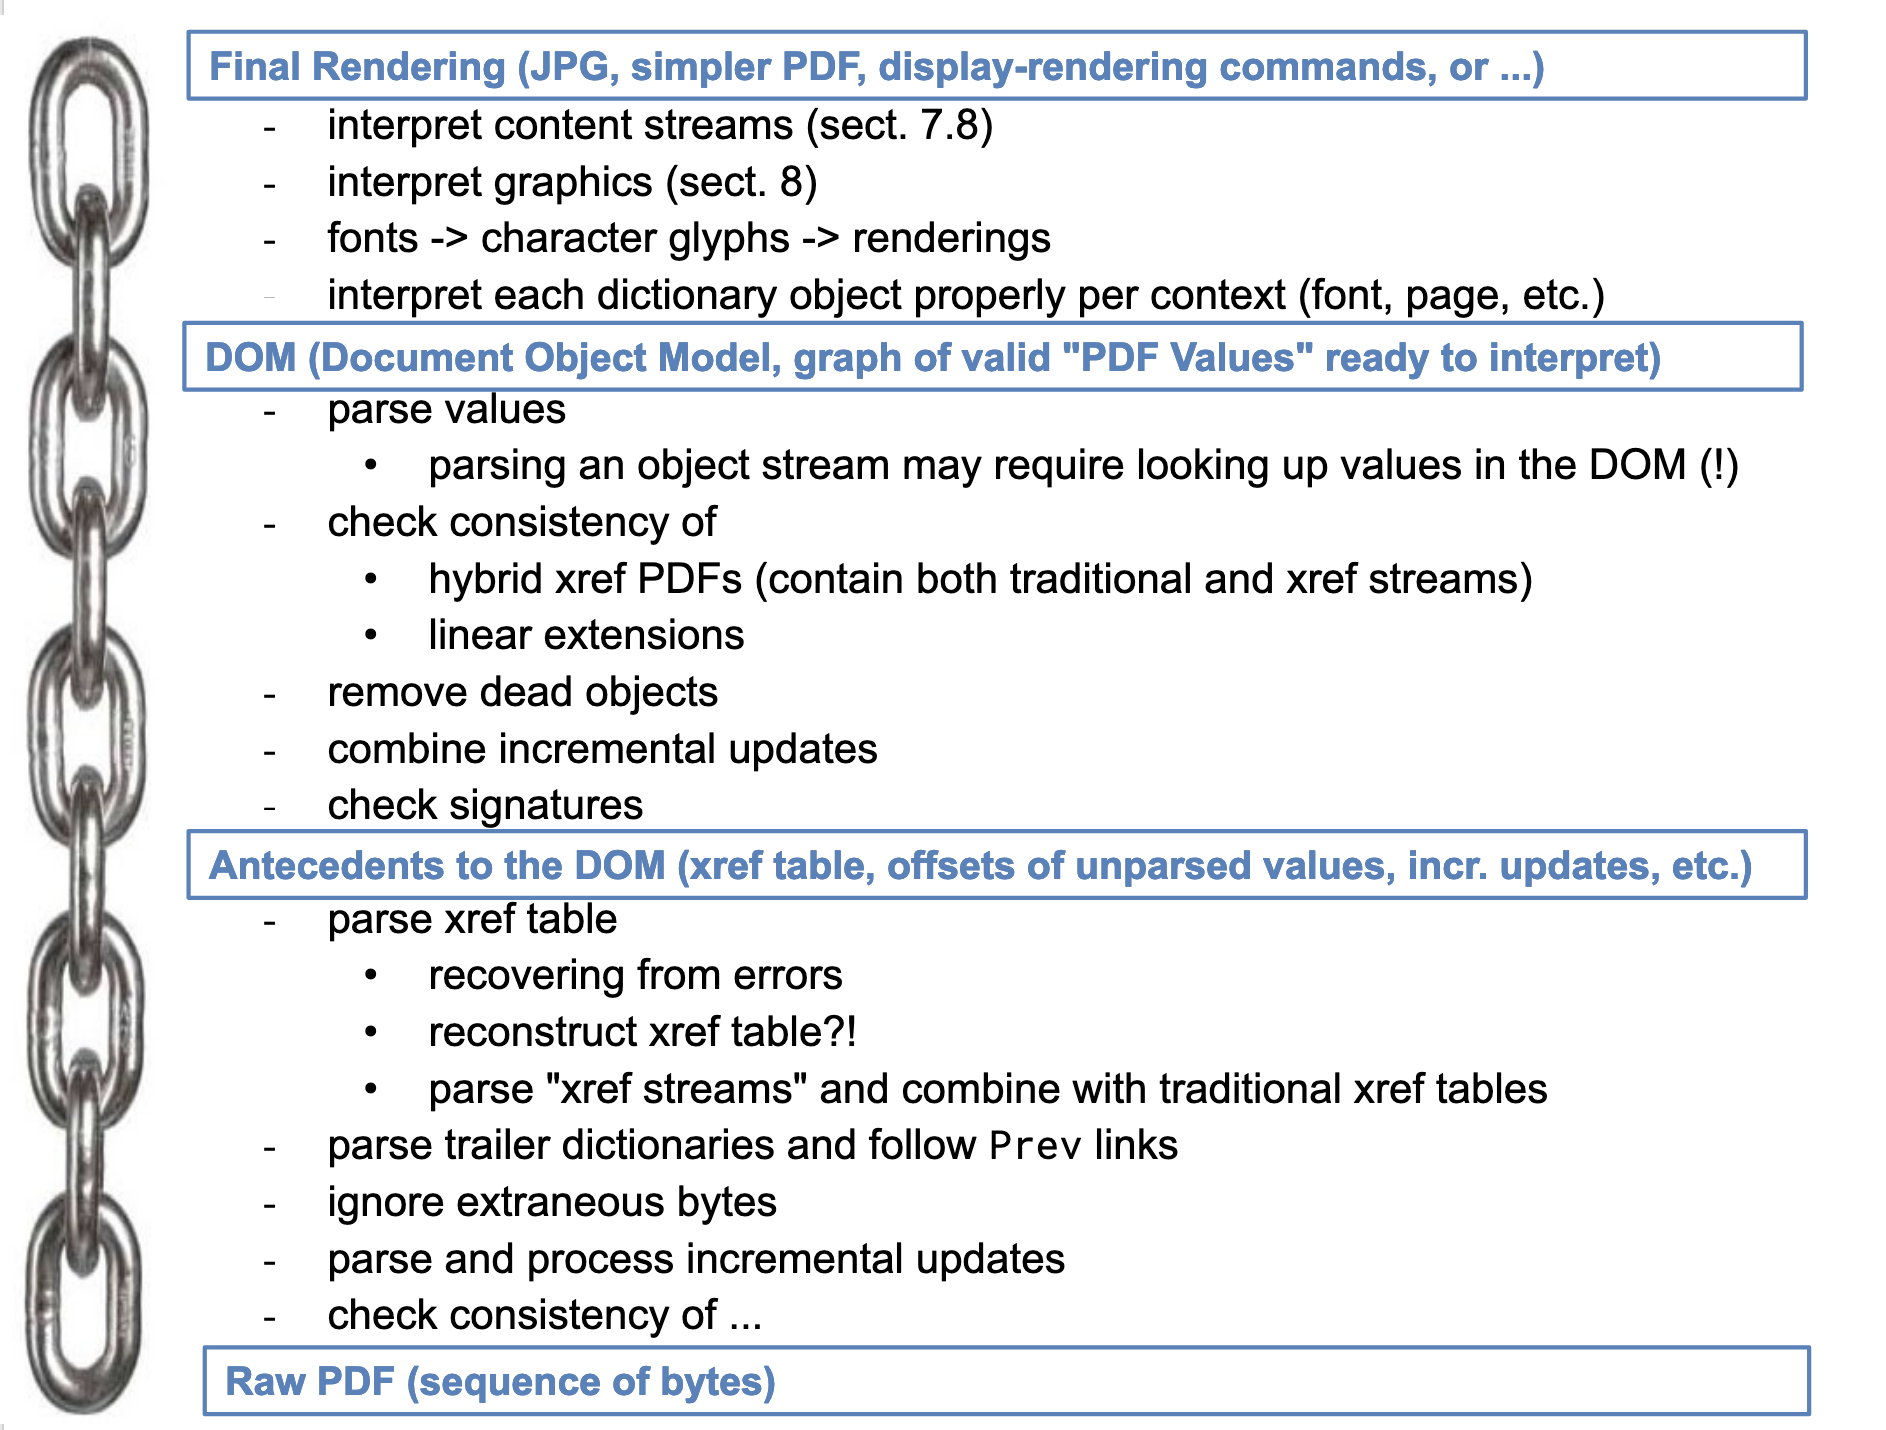
\includegraphics[width=0.8\linewidth]{figures/trustchain-diagram.png}
    \caption{The PDF Trust Chain diagrammed.}
    \todo{make diagram prettier!}
    \label{fig:pdf-trust-chain}
\end{figure}

We have touched upon the complexities of parsing
PDF, but to appreciate these, one has to understand the
dependencies and interactions between the features.
In \cref{fig:pdf-trust-chain} we show the main components diagrammatically.
To briefly sketch what's going on here:
\begin{itemize}
\item Phase 1: Find and parse both the PDF header and the PDF trailer.

\item Phase 2: using information from Phase 1, we find and parse any incremental
  updates.

\item Phase 3: \todo{...}
  
\item Phase 4: \todo{...}
  
\item Phase 5: \todo{...} The result is the candidate DOM, the candidate DOM is
  a mapping \lstcd{ObjId -> PdfValue}.
\item Phase 6: This phase takes the candidate DOM and verifies that it
  represents a sensible Document Tree per the PDF Standard.  E.g., all indirect
  objects are in the candidate DOM, no unexpected recursion, etc.
\item Render Phase: we can now render the validated DOM, or parts thereof, to
  whatever display or graphic format we choose.
\end{itemize}

Note that phases 2, 3, 4 and 5
all require inputs from the previous phase to enable them to know where and
how to parse further segments of the PDF input file.
%
Note this: an implementation \emph{might} merge phases 1-4 into single phase
and give a \emph{semblance} of simplicity, but our argument (in what
follows---particularly in \cref{sec:single-pass-problems}---is that
such an implementation will be overly complex and
it will be a near insurmountable task to assure that such an implementation
terminates for all input files.

% Only after Phase 5, have we correctly constructed a 'candidate' DOM (Document
% Object Model) where we have a mapping of Object Identifiers to PDF Values.

Although verifying Phase 5 is both difficult and tedious
(\todo{...; say something re the Arlington DOM model? Paper?})
and the Render phase has many complications of its own (fonts are
a special challenge, etc.), in this paper we focus on Phases 1-4.
We call these phases the pre-DOM parsing/computation, and if anything
goes wrong pre-DOM, lots can go wrong, the wrong DOM may be rendered, etc.!
% ^ awkward, rewrite

The attentive reader will note that we have another instance of a \emph{Trust
Chain}.  The later phases of the parsing process are \emph{completely
dependent} upon the earlier phases to properly parse and interpret the PDF
file.

We think it is important to understand PDF parsing in terms of this
\emph{Trust Chain} because
%
(1) it highlights the presence of the many ``dependent'' parsers (or phases)
in PDF processing.
%
(2) it highlights the importance of ensuring the pre-DOM parsing, data integrity relationships and
computation (the base of our Trust Chain) is correct and secure.
%
(3) it reminds us that the integrity of the DOM cannot be verified
independently of the lower levels.
(4) it shows that PDF parsing, although uniquely complex, is an instance of
a general concept.

